\documentclass[manuscript,review,anonymous]{acmart}
\usepackage{caption}
\usepackage{subcaption}
\usepackage{hyperref}

% NOTE: Good things
%  - what is iterative prompting? "Like auto-complete but less limited" - hmm, maybe
%  - sell more main idea: can do much with very limited set of commands / via auto-complete
%  - paper is convincing in that this works for SQL-like queries (maybe not general purpose, but this is good)
%  - journalism is a good focus / but needs to deemphasize this a bit because of the study
%  - #1 Limited language for data exploration (what is included / excluded / essential / could be added)
%  - #2 Iterative prompting - what's new? people can get to all programs via '.' and up/down/enter.

% NOTE: Random
%  - How choices were made?
%  - Terminology: data analysis / data exploration / data visualization - what is the goal of the system? (fair enough)
%    (it's not about writing charts - just about getting the right data - we have limited charting functionality,
%     one could integrate with Vega, or do future work based on iterative prompting)
%  - Technical details - you can only create valid programs!! (it's contextual)
%  - Minor: what was "demo" at the start of a session
%  - Table 1 vs. Table 2 numbers of participants
%  - What data quality is needed to make this work?
%  - "Magic Escalator of Knowledge" - remove bs?
%  - Clarify how we support 3D cubes (no unified API); mention "done by intern in X weeks"

% TODO
%   - SAY SOMEWHERE: choose function *and* specify arguments via auto-complete
%   - ADD: table of all available operations? (shorten introduction)

% NOTE: Contribution
%  - What is the exact goal? (so that it can be compared with R, Python, Vega-Lite, Tableau)
%  - How the design goals were generated? (not by talking to journalists)
%  - "notebooks are messy" - not arguing we can fix that

% NOTE: Motivation
% - what if you could write the whole program using auto-complete?

% Explain type providers a bit more (we say what it does, but not much about what
% it is - give dynamic typing in a static language)
%
% The 'then' operation was mysterious - can we add one line explanation to the operations?
% (yes we can and we should totally do that)




% \usepackage{xspace}
\usepackage{fancyvrb}
% \usepackage{inconsolata}
\usepackage{xcolor}
\usepackage{tikz}
\newcommand*{\priority}[1]{\begin{tikzpicture}[scale=0.12]%
   \draw (0,0) circle (1);
   \fill[fill opacity=1,fill=black] (0,0) -- (90:1) arc (90:90-#1*3.6:1) -- cycle;
   \end{tikzpicture}}
\newcommand*{\priorityc}[1]{
\resizebox{0.8em}{0.8em}{
 {\protect\tikz{ \protect
   \draw[line width=1mm, black] (0,0) circle (1); \fill[fill opacity=1,fill=black] (0,0) -- (90:1) arc (90:90-#1*3.6:1) -- cycle;
   } }}}
%
\definecolor{kvdclr}{rgb}{0.3,0.0,0.8}
\DefineVerbatimEnvironment{thegamma}{Verbatim}{fontfamily=zi4,numbers=left,xleftmargin=6mm,fontsize=\small,commandchars=\\\{\}}
% %\newcommand{\kvd}[1]{\textcolor{kvdclr}{#1}}
\newcommand{\kvd}[1]{\textbf{#1}}
\newcommand{\ikvd}[1]{{\fontfamily{zi4}\selectfont\small #1}}
% \usepackage{balance}       % to better equalize the last page
% \usepackage{graphics}      % for EPS, load graphicx instead
% \usepackage[T1]{fontenc}   % for umlauts and other diaeresis
% \usepackage{txfonts}
% \usepackage{mathptmx}
% \usepackage[pdflang={en-US},pdftex]{hyperref}
% \usepackage{color}
% \usepackage{booktabs}
% \usepackage{textcomp}

\setcopyright{acmwhatever}
\copyrightyear{2020}
\acmYear{2020}
%\acmDOI{10.1145/1122445.1122456}
\acmConference[Woodstock '18]{Woodstock '18: ACM Symposium on Neural
  Gaze Detection}{June 03--05, 2018}{Woodstock, NY}
\acmBooktitle{Woodstock '18: ACM Symposium on Neural Gaze Detection,
  June 03--05, 2018, Woodstock, NY}
\acmPrice{15.00}
%\acmISBN{978-1-4503-XXXX-X/18/06}

\begin{document}
\title{Iterative Prompting: Programmatic Data Exploration for Non-programmers}

\author{Tomas Petricek}
\email{t.petricek@kent.ac.uk}
\affiliation{%
  \institution{University of Kent}
  \city{Canterbury, UK}
}
%\renewcommand{\shortauthors}{Trovato and Tobin, et al.}

\begin{abstract}
  Data exploration tools based on code have many desirable characteristics. They can easily access
  a wide range of different data sources, result in reproducible scripts and encourage users to
  reuse and modify existing code. Unfortunately, most programming tools require expert
  coding skills. Can we make data exploration based on code accessible to non-experts?
  %
  We present The Gamma, a novel text-based data exploration environment that answers the question in
  the affirmative. The Gamma is based on a novel interaction principle, \emph{iterative prompting},
  which lets users create transparent and reproducible scripts without writing code. The Gamma lowers
  the barrier to entry and learning from previously created data analyses. We evaluate the usability
  of The Gamma through a user study on non-technical employees of a research institute.
  %
  Our work shows that we may not need to shy away from code in order to build accessible,
  reproducible and transparent tools that will allow a broad audience to benefit from the
  rise of open data.
\end{abstract}

\begin{CCSXML}
<ccs2012>
   <concept>
       <concept_id>10003120.10003121.10003124</concept_id>
       <concept_desc>Human-centered computing~Interaction paradigms</concept_desc>
       <concept_significance>500</concept_significance>
       </concept>
   <concept>
       <concept_id>10011007.10011006.10011050.10011017</concept_id>
       <concept_desc>Software and its engineering~Domain specific languages</concept_desc>
       <concept_significance>300</concept_significance>
       </concept>
   <concept>
       <concept_id>10011007.10011006.10011066.10011069</concept_id>
       <concept_desc>Software and its engineering~Integrated and visual development environments</concept_desc>
       <concept_significance>500</concept_significance>
       </concept>
 </ccs2012>
\end{CCSXML}

\ccsdesc[500]{Human-centered computing~Interaction paradigms}
\ccsdesc[500]{Software and its engineering~Integrated and visual development environments}
\ccsdesc[300]{Software and its engineering~Domain specific languages}
\keywords{data exploration; end-user programming; data journalism; programming languages; type providers}

\maketitle

\begin{figure}
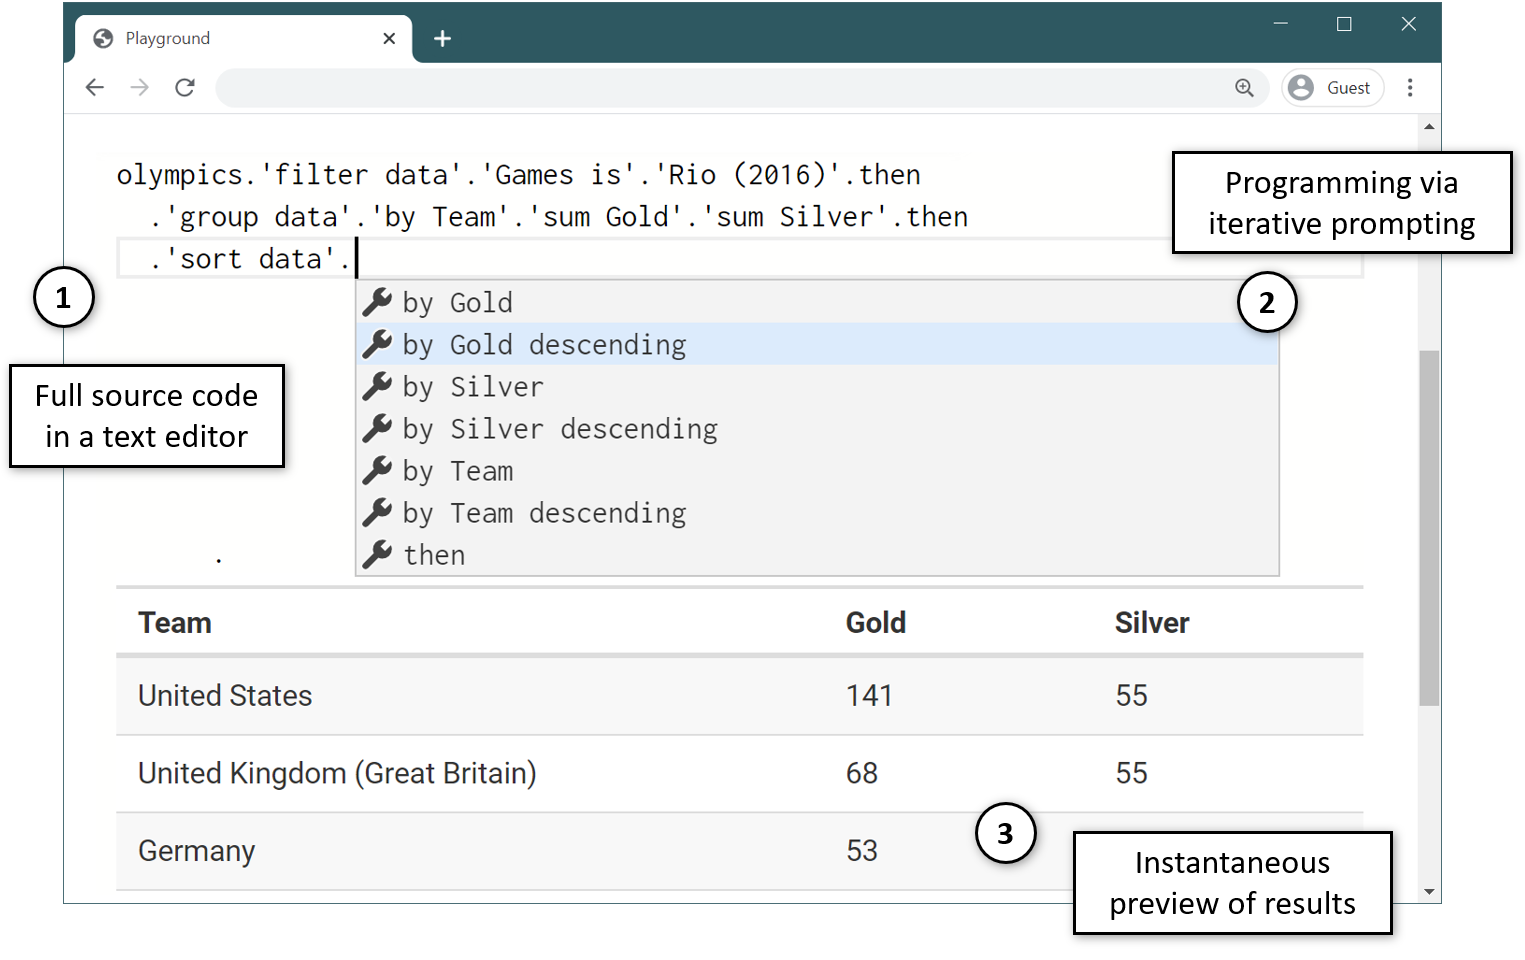
\includegraphics[width=.63\columnwidth]{figures/thegamma-annot}
\vspace{-0.5em}
\caption{Obtaining teams with the greatest number of gold medals from Rio 2016
Olympics with a reproducible The Gamma script (1), contextual iterative prompting mechanism
offering ways of sorting the data (2) and an instant preview of results (3).}
\label{fig:thegamma}
\vspace{-0.5em}
\end{figure}

% ==================================================================================================

\section{Introduction}
Despite the advances on visual tooling, programmatic data exploration remains the choice of
expert analysts. It is flexibile, offers greater reusability and leads to transparent
analyses. We aim to make programmatic data exploration accessible to a wider range of users.
The design of a data exploration tool that would make this possible poses a number of challenges.
First, the tool needs to have a low barrier to entry. Second, it needs to support a wide
range of data sources in a uniform way. Third, the users should be able to learn how to use the
tool by looking at existing data analyses.

We contribute The Gamma, a text-based data exploration environment for non-experts. The Gamma
is based on a single, easy to understand interaction principle and provides a uniform
access to a range of data sources including data tables, graph databases and data cubes.
The resulting analysis is a transparent script that can be followed to reproduce the
result from scratch. This allows learning from existing analyses and encourages readers
to engage with data.

\subsubsection*{Iterative Prompting}
The main contribution of our work is the \emph{iterative prompting} interaction principle,
which makes it possible to construct all valid data exploration scripts by repeatedly choosing
an item from a list of options offered through auto-complete. The design favors \emph{recognition
over recall} and allows non-programmers to write entire scripts without typing code and without
learning a programming language first. Yet, it still results in transparent and reproducible code.
In other words, iterative prompting turns auto-complete from a programmer
assistance tool into a non-expert programming mechanism. A crucial feature is that iterative
prompting only offers operations that are valid in a given context and that it offers all such
operations; it is both correct and complete.

\subsubsection*{Data Exploration}
The Gamma focuses on data exploration of the kind illustrated in Figure~\ref{fig:thegamma}.
The user accesses data available in a structured format. They make several experiments to find an
interesting way of looking at the data, e.g.~by applying different aggregations or filters. They
may choose to view the results as a table or a basic chart before publishing their analysis. The
Gamma makes such programmatic data exploration simple enough for non-experts, but scraping and
cleaning of messy data or building custom data visualizations is currently outside of the scope of
our work. Exposing those using iterative prompting remains an interesting and worthwhile future
challenge.

\subsubsection*{Paper Overview}
The Gamma is available (non-anonymously) at \url{http://thegamma.net},
both as a JavaScript library and a hosted data exploration service. In this paper, we describe and
evaluate the design principles behind the project\footnote{This paper is 11 pages (5500 words),
without citations, to be commensurate with the size of the contribution.}:

\begin{itemize}
\item We introduce the iterative prompting principle in The Gamma
  and show how it can be used for querying of distinct data sources including data tables, graph
  databases and data cubes (Section~\ref{sec:overview}).

\item We evaluate the system through a number of case studies (Section~\ref{sec:cases})
  and a user study (Section~\ref{sec:study}), which confirms  that non-programmers can use The Gamma
  to construct non-trivial data queries.

\item We reflect how our design lowers barriers to entry, supports learning without experts and offers a
  complete and correct program construction method (Section~\ref{sec:discuss}).
\end{itemize}

% ==================================================================================================

\section{Related Work}

The key contribution of our work is that it develops a new, fundamentally different, way of using the
established auto-completion mechanism. Unlike most past work dating back to Kaiser~\cite{assistants},
we do not view it as a programmer assistance tool. Instead, we turn it into an interaction mechanism
through which non-experts can create entire programs. We build on recent research on information-rich
programming \cite{inforich} and aim to make those advances available to non-programmers
\cite{enduser,smallmatter}, in the context of data exploration as done, for example, by journalists
\cite{ddj}. Our work features a novel combination of characteristics in that our iterative prompting
interaction principle (i) is centered around editing and understanding of code,
(ii) reduces conceptual complexity to a single basic kind of interaction, yet (iii) it is
correct and complete in that it can be used to construct all meaningful queries for a variety
of data sources.

\subsubsection*{Code Completion for Data Science}

A key component in The Gamma is the use of auto-complete for offering possible operations.
Our work follows type providers \cite{inforich,fsdata}, which integrate external data into a
static type system of F\#, allowing the use of auto-completion; for querying data tables, we utilize
the theory developed by Petricek \cite{dotdriven}. The key difference in our work is that The Gamma
can be used without a programming language expertise.

Most similar to our approach are tools that make recommendations when users begin interacting
with data. Those based on machine learning-based code completion for domain specific languages \cite{predictive,proactive}
differ in that they do not guarantee completeness, i.e.~it is unclear whether the user can create all possible
scripts. Approaches based on natural language are effective \cite{eviza,codemend}, but hide the
underlying structure and do not help the user understand it. Conversational agents \cite{iris}
share similar characteristics, except that the construction process is iterative.

Code completion based on machine learning or statistical
methods \cite{mlcomplete,statcomplete} also exists for general-purpose programming languages used
by data scientists such as Python \cite{pythia}, providing assistance to expert programmers.
Finally, DS.js \cite{dsjs} is interesting in that it enables querying of data on the
web. It uses JavaScript, but with rich contextual code completion.

\subsubsection*{Notebooks and Business Intelligence Tools}

Notebooks such as Jupyter \cite{jupyter}, which allow combining source code with commentary and
visual outputs, are widely used by data scientists, but require expert programming skills.
The Gamma targets non-experts, but could also be integrated with a multi-language notebook system
\cite{wrattler}.
%
Spreadsheets, business intelligence tools \cite{tableau,powerbi} and other visual data analytics
tools \cite{control,vizdom} do not involve programming, but require mastering a complex GUI.
In contrast, The Gamma is based on a single kind of interaction, through which all available operations
can be completed. Several systems \cite{potter,wrangler,lyra} record interactions with the GUI
as a script that can be modified by the user. Unlike in The Gamma, the source code does not
guide the user in learning how to use the system.

\subsubsection*{Easier Programming Tools}
We aim to build an easy to use and learn programming system. Many approaches to this
goal have been tried. Victor \cite{principle} introduced design principles that
inspired many to build live programming systems \cite{review,liveroad,lighttable} that give
immediate feedback to help programmers understand how code relates to output and
exploratory systems \cite{variolite,exploratory} that assist with completing open-ended tasks.
A system combining textual language with visualization also exists for graph querying \cite{guess}.
To avoid difficulties with editing code as text, some systems use structured editors~\cite{structure-based,livenut,lamdu}.
In Subtext \cite{subtext,directprog} the language itself is co-designed with the editor to make
the interactions with code more natural. The Gamma is live in that our editor gives an instant
preview of the results.
%
Many systems simplify programming by offering high-level abstractions,
e.g.~for interactive news articles \cite{idyll}, statistical analyses \cite{tea}
or interactive data visualization \cite{interactionviz,vegalite}. The Gamma exposes a number
of data sources through high-level abstractions that support iterative prompting, but support
for tasks other than querying remains furture work.

\subsubsection*{Programming without Writing Code}
There are two main approaches to programming where
the user does not write code. In programming by example \cite{byexample}, the user gives
examples of desired results. This has been used, e.g.~for specifying data transformations
in spreadsheets and data extraction \cite{spreadsheetpbe,flashextract}.
In direct manipulation \cite{direct}, a program is specified by directly interacting with the
output. This has been used in the visual domain \cite{sketchnsketch}, but also for data querying
\cite{dynamicq,vlang}. The VQE language~\cite{visage} also considers how to allow code reuse and
modification in this context. Direct manipulation can also support data exploration by letting
users partially edit queries,~e.g. by changing quantifiers as in DataPlay~\cite{dataplay}.

\subsubsection*{Gestures and Data Entry}
Although our focus is on program construction, our work can be positioned in the
broader context of input methods. Akin to Dasher \cite{dasher}, our system provides a way of
navigating through a complete space of options, while on-screen feedforward \cite{octopocus} allows
efficient selection in gesture-based interfaces. Those provide compelling alternatives to
auto-completion menus, although the efficiency of input methods is typically not an issue in programming.


\begin{figure}[b]
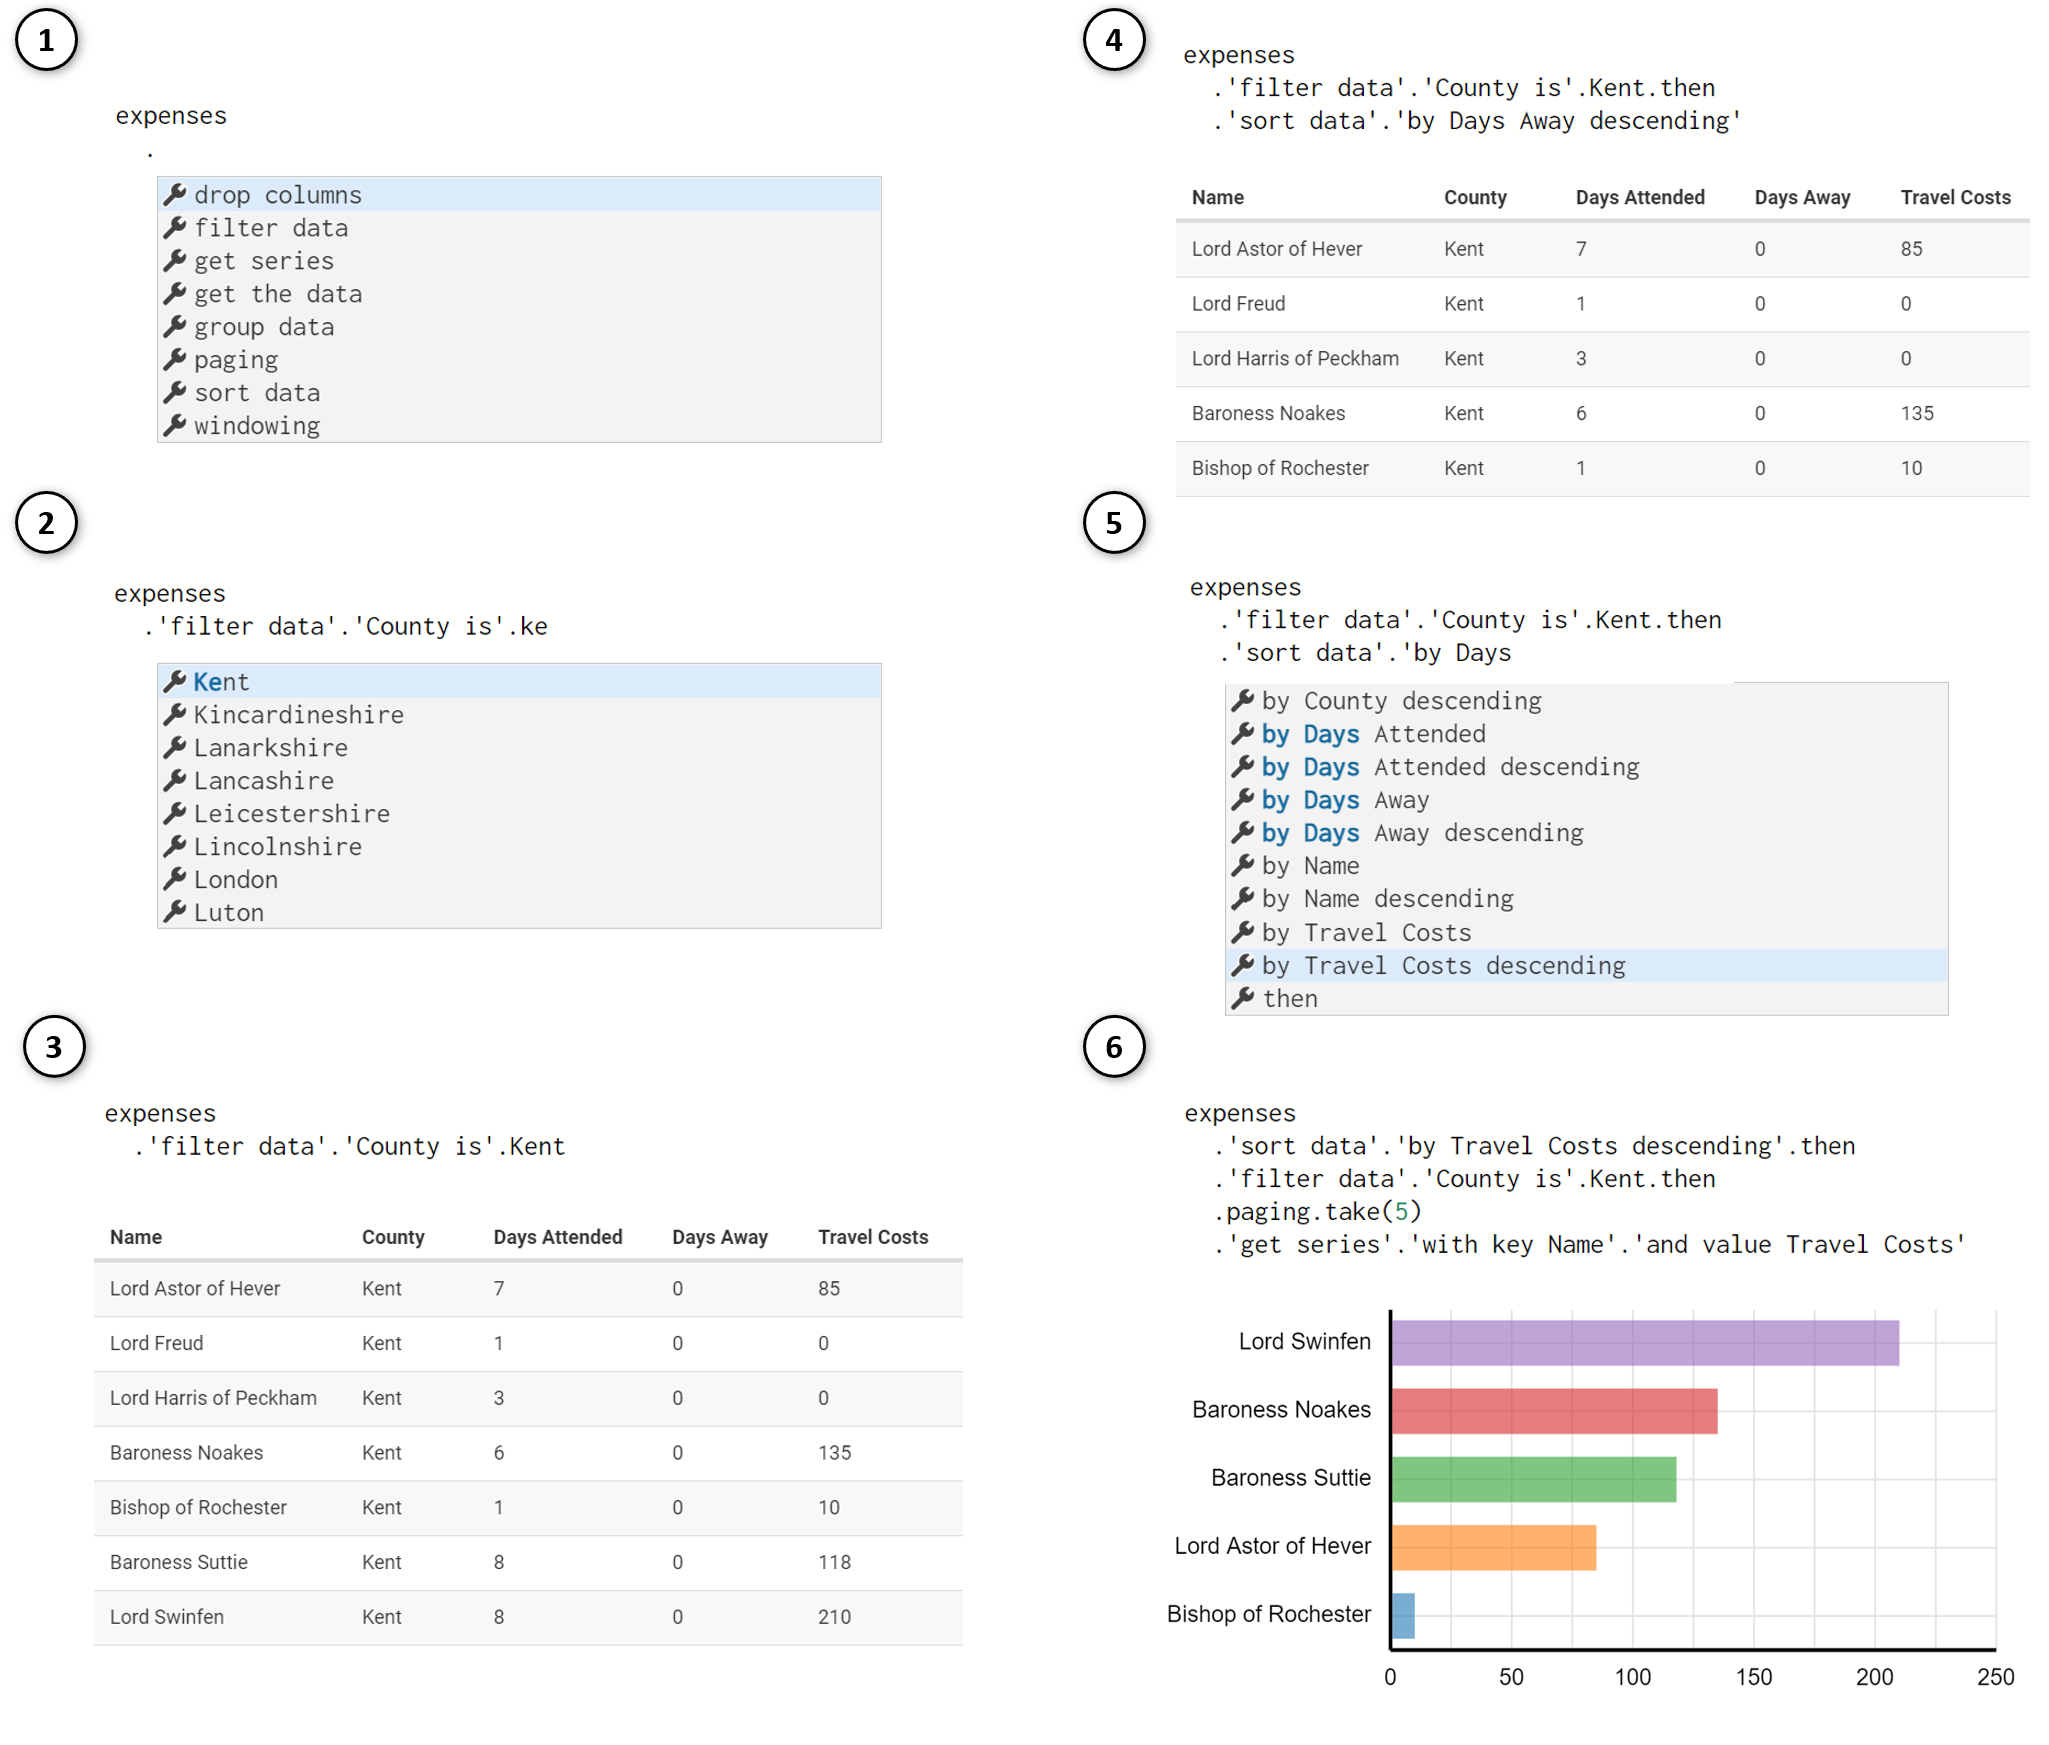
\includegraphics[width=0.94\columnwidth]{figures/thegamma-walk}
\caption{Constructing a script that charts the top 5 members of the House of Lords for Kent, based
on their travel costs.}
\label{fig:walkthrough}
\end{figure}

% ==================================================================================================

\section{Overview}
\label{sec:overview}

The Gamma aims to make text-based data exploration easy enough for non-experts. The aim is
motivated, in part, by the desirable properties of text-based data exploration tools such
as transparency, reproducibility and learnability and, in part, by an aim to explore an
unexplored point in the design space of data exploration tools. Although various efforts
make text-based programming easier, most systems that target non-experts shy away from code.

The Gamma is a text-based data exploration environment that allows non-experts explore data using
iterative prompting -- by repeatedly selecting an item from an auto-complete list. The study
presented in Section~\ref{sec:study} confirms that the kind of data exploration shown in the next
section can, indeed, be successfully done by non-experts.
%
\subsection{Querying Travel Expenses}
\label{sec:overview-walk}

The walkthough in Figure~\ref{fig:walkthrough} shows a typical task completed using The Gamma.
A data analyst from Kent is exploring travel expense claims by members of the House of Lords published
by the UK government \cite{lords}. The following shows a subset of the data in the CSV format:


\begin{thegamma}
\textbf{Name, County, Days Attended, Days Away, Travel Costs}
Lord Adonis, London, 8, 0, 504
Baroness Afshar, Yorkshire, 2, 0, 0
Lord Alderdice, Oxfordshire, 3, 0, 114
Lord Alli, London, 5, 0, 0
\end{thegamma}
% Baroness Amos, London, 3, 0, 0

\noindent
The analyst imports the file through a web interface, the environment is initialised with code
that refers to the imported data as \ikvd{expenses} and she starts exploring the data using the type provider for tabular data (Section~\ref{sec:overview-tps}):

\begin{enumerate}
\item The analyst types `.' (dot) to trigger auto-completion on \ikvd{expenses}. The type provider
  offers a list of operations that the analyst can perform. To find House of Lords
  members from Kent, the analyst chooses \ikvd{filter data}.

\item The analyst is offered a list of columns based on the schema of the tabular data and choses
  \ikvd{County is}.  She is then offered a list of counties in the data set and types \ikvd{ke} to
  search for Kent and she selects \ikvd{Kent}.

\item The Gamma evaluates the code on-the-fly and shows a
  preview of results. The analyst now sees a table with House of Lords members from Kent.
  She wants to see if there are any members who missed any House sessions.

\item The analyst finishes specifying the (possibly compound) sorting key by choosing \ikvd{then}
  and is offered the same list of querying operations as in the first step. She selects
  \ikvd{sort data} followed by \ikvd{by Days Away descending}.

\item The analyst sees that there are no reported ``days away'' and decides to compare
  travel costs. She hits the backspace key a number of times, is offered the list
  of keys again and selects \ikvd{by Travel Costs descending}.

\item The analyst chooses \ikvd{then} and is,
  again, offered the list of querying operation. She uses \ikvd{paging} to get top 5 records,
  which requires typing \ikvd{5} as the argument. She then uses the \ikvd{get series} operation
  to obtain a data series associating travel expenses with a name, which is automatically
  visualized using a bar chart.
\end{enumerate}

\noindent
The constructed code is not unlike an SQL query, except that the whole script is constructed using
iterative prompting, by repeatedly selecting one of the offered members. Those represent both
operations, such as \ikvd{sort by} and arguments, such as \ikvd{Kent}. The only exception
is when the analyst needs to type the number \ikvd{5} to specify the number of items to take.

\subsection{The Gamma Programming Environment}
\label{sec:overview-lang}

A program in The Gamma is a sequence of commands. A command can be either a variable declaration
or an expression that evaluates to a value such as a data table or a chart.
An expression is a reference to a data source followed by a chain of member accesses.
A member can be either an ordinary member such as \ikvd{paging} or an operation which takes a
list of parameters enclosed in parentheses as in \ikvd{take(5)}.
Names with non-alphanumerical characters are escaped using quotes.

The Gamma uses a type system to infer what members are available at a given point in a chain.
Each expression has a type with a list of members that, in turn, have their own types.
The types are not built-in, but are generated by type providers for individual data sources.
The programming environment for The Gamma is based on the Monaco editor \cite{monaco}. When the user types `.'
the editor triggers auto-completion and retrieves a list of available members based on the type
information. The Gamma evaluates scripts on-the-fly and shows a preview as
illustrated in Figure~\ref{fig:thegamma}.

There is a handful of situations where The Gamma does not yet fully support the iterative prompting
principle. First, it allows operations with parameters such as \ikvd{take(5)}. This is currently
needed when writing a query that skips or takes the first N elements from a table. Second,
The Gamma allows the user to declare (immutable) variables using \ikvd{let}. This is not needed
for basic data exploration, but allows advanced users to better structure more complex code.

\begin{figure}
\centering
\begin{subfigure}[b]{0.5\textwidth}
  \centering
  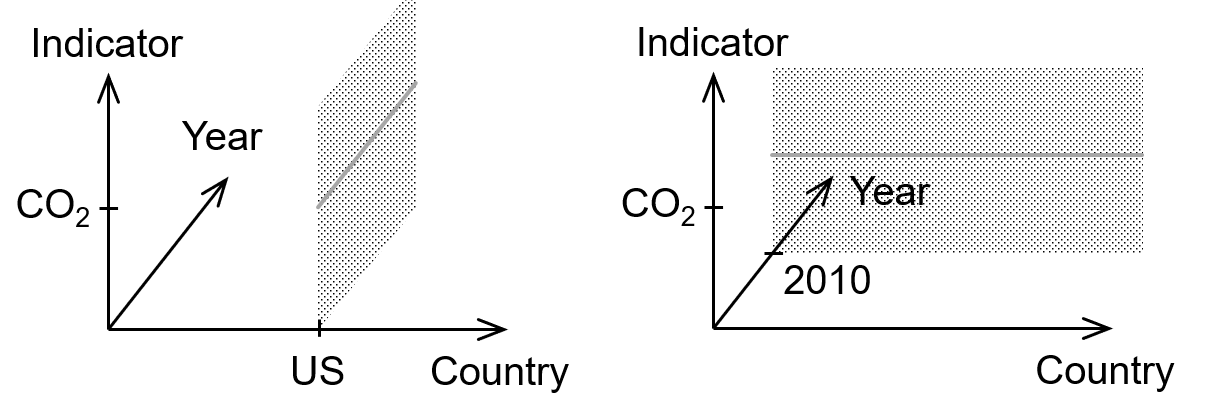
\includegraphics[scale=0.24]{figures/cubetp}
  \vspace{0.5em}
  \caption{Exploring World Bank data using the data cube type provider, users
    choose values from two dimensions to obtain a data series.}
  \label{fig:cubetp}
\end{subfigure}
\hfill
\begin{subfigure}[b]{0.45\textwidth}
  \centering
  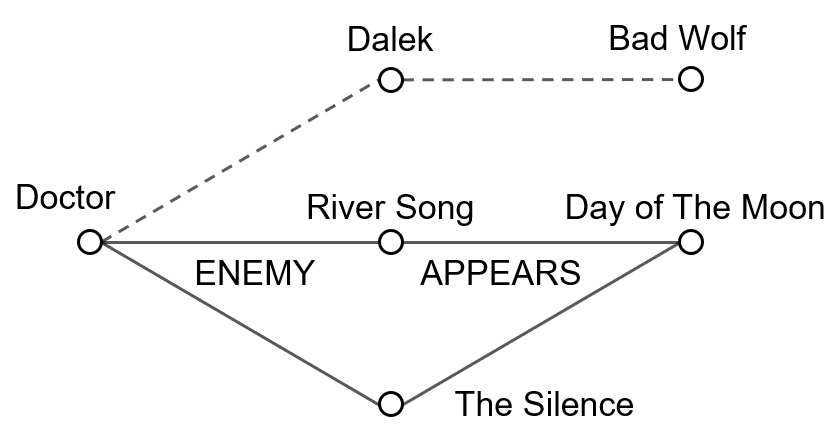
\includegraphics[scale=0.27]{figures/graphtp}
  \caption{To query graph data, the user specifies a path through the data, possibly with
    placeholders to select multiple nodes.}
  \label{fig:graphtp}
\end{subfigure}
\vspace{-0.5em}
\caption{Design of type providers for exploring data cubes and graph databases.}
\label{fig:tps}
\end{figure}

\subsection{Type Providers for Data Querying}
\label{sec:overview-tps}

The Gamma can be extended to support any data source by implementing a \emph{type provider},
which defines a domain specific language for exploring data of a particular kind.
A type provider generates object types with members (such as \ikvd{paging} or \ikvd{Kent})
that are accessed via iterative prompting. We describe type provider for exploring data cubes
(inspired by Syme et al. \cite{inforich}), tabular data (based on theory developed
by Petricek \cite{dotdriven}), and graph databases.

\subsubsection*{Data Cube Type Provider}
Our first type provider allows users to explore data cubes, which are multi-dimensional
arrays of values. For example, the World Bank collects a range of indicators about many countries
each year while the UK government expenditure records spending for different government services,
over time, with different adjustments:

\begin{thegamma}
worldbank.byCountry.'United States'.'Climate Change'.'CO2 emissions (kt)'
expenditure.byService.Defence.inTermsOf.GDP
\end{thegamma}

\noindent
The dimensions of the \ikvd{worldbank} cube are countries, years and indicators, whereas the dimensions
of \ikvd{expenditure} are government services, years and value type (adjusted, nominal,
per GDP).  Figure~\ref{fig:cubetp} how the provider allows users to slice the data cube.
Choosing \ikvd{byCountry.\textquotesingle United States\textquotesingle},
restricts the cube to a plane and selecting \ikvd{\textquotesingle CO2 emissions (kt)\textquotesingle}
then gives a series with years as keys and emission data as values. Similarly, we could first filter the
data by a year or an indicator. The same mechanism is used to select UK government spending on
defence in terms of GDP.
%  As there is no widely used standard format for data cubes, adding another data cube to The Gamma
% currently requires implementing a new type provider.

\subsubsection*{Tabular Data Type Provider}

Our second type provider allows users to construct queries to explore data in tabular formats.
Unlike the data cube provider, the provider for tabular data does not just
allow selecting a subset of the data, but it can be used to construct SQL-like query. Consider
the example from Figure~\ref{fig:thegamma}:

\begin{thegamma}
olympics.'filter data'.'Games is'.'Rio (2016)'.then
  .'group data'.'by Team'.'sum Gold'.'sum Silver'.then
  .'sort data'.'by Gold descending'
\end{thegamma}

\noindent
The example queries a table that records individual medals awarded in Olympic games.
The chain constructs a query that selects rows corresponding to the Rio 2016 Olympics and then
calculates total number of gold and silver medals for each team (country) before sorting the data.
%
When using the provider, the user specifies a sequence of operations. Members such as
\ikvd{\textquotesingle filter data\textquotesingle} or \ikvd{\textquotesingle group data\textquotesingle}
determine the operation type. Those are followed by operation parameters. For example, when grouping
data, we first select the key and then choose a number of aggregations to calculate over the group.
Unlike SQL, the provider only allows users to choose from pre-defined aggregations such as
calculating the sum, average or the number of distinct values.
Section~\ref{sec:cases} shows that this is sufficient to construct a range of practical queries.



\subsubsection*{Graph Database Type Provider}
Our third type provider allows users to explore data from graph databases, which store
nodes representing entities and relationships between them.
The following example explores a database of Doctor Who characters and episodes. It retrieves
all enemies of the Doctor that appear in the Day of the Moon episode:

\begin{thegamma}
drwho.Character.Doctor.'ENEMY OF'.'[any]'.'APPEARED IN'.'Day of the Moon'
\end{thegamma}

\noindent
We start from the \ikvd{Doctor} node and then follow two relationships. We use
\ikvd{\textquotesingle ENEMY OF\textquotesingle.\textquotesingle [any]\textquotesingle}
to follow links to all enemies of the Doctor and then specify
\ikvd{\textquotesingle APPEARED IN\textquotesingle}
to select only enemies that appear in a specific episode. The result appears in
in Figure~\ref{fig:graphtp}.
%
The provider works with any graph database and generates members automatically, based on the
data. In the above, \ikvd{ENEMY OF} and \ikvd{APPEARED IN} are labels
of relations and \ikvd{Doctor} and \ikvd{Day of the Moon} are labels of nodes. The
\ikvd{[any]} member defines a placeholder that can be filled with any node with the specified
relationships. The results returned by the provider is a table of properties of all nodes
along the specified path. As illustrated by an example discussed in Section~\ref{sec:cases},
the returned table can be further queried using the tabular data type provider.

\begin{figure}[t]
\vspace{-0.5em}
\centering
\begin{subfigure}[b]{0.49\textwidth}
  \centering
  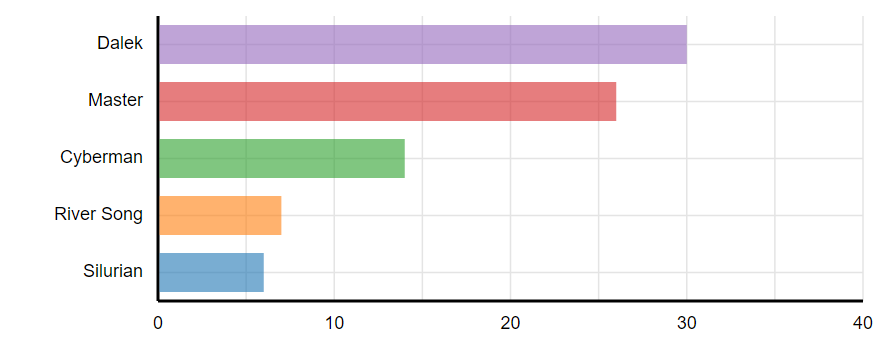
\includegraphics[width=0.96\columnwidth]{figures/cases-dr}
  \caption{Exploring Dr Who graph database by composing type providers}
  \label{fig:cases-dr}
\end{subfigure}
\hfill
\begin{subfigure}[b]{0.49\textwidth}
  \centering
  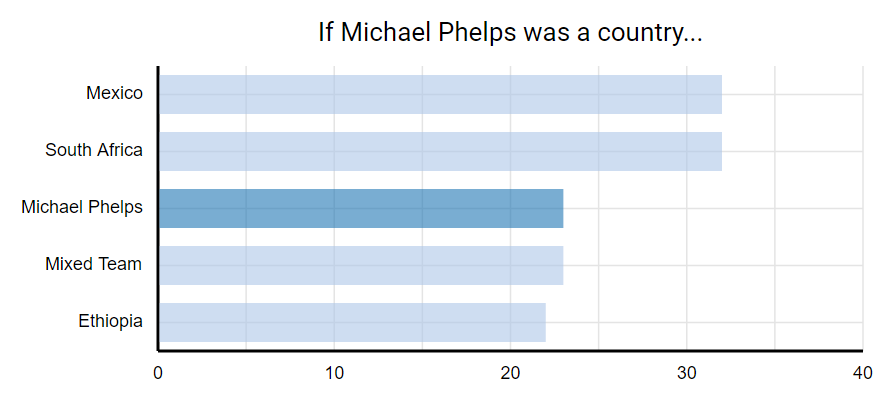
\includegraphics[width=0.96\columnwidth]{figures/cases-mp}
  \caption{Exploring Olympic medallists using tabular data type provider}
  \label{fig:cases-mp}
\end{subfigure}
\vspace{-0.5em}
\caption{Charts produced by two case studies of using The Gamma.}
\label{fig:cases}
\vspace{-0.5em}
\end{figure}

% ==================================================================================================

\section{Case Studies}
\label{sec:cases}

The Gamma aims to simplify programmatic data exploration while keeping enough expressive power
to allow users to create interesting data explorations. In this section, we consider two case
studies that evaluate expressivity and show what can be achieved using the simple
iterative prompting principle\footnote{Available (non-anonymously) at:
\url{http://gallery.thegamma.net/86/} and  \url{http://gallery.thegamma.net/87/}, respectively.}.
We used The Gamma for larger projects exploring the UK government expenditure, activities of a
research institute adn Olympic medal winners\footnote{Available (non-anonymously)
at \url{http://turing.thegamma.net} and \url{http://rio2016.thegamma.net}}.

\subsubsection*{The Most Frequent Doctor Who Villains}
Our first case study uses a graph database with data from the Dr Who series. It lists Dr Who villains
by the number of episodes in which they appear. This case study is interesting as it
combines the graph database provider for fetching the data with the tabular data provider for
summarization:

\begin{thegamma}
drWho.Character.Doctor.'ENEMY OF'.'[any]'.'APPEARED IN'.'[any]'.explore
  .'group data'.'by Character name'.'count distinct Episode name'.then
  .'sort data'.'by Episode name descending'.then
  .paging.take(8).'get series'.'with key Character name'.'and value Episode name'
\end{thegamma}

\noindent
Line 1 use the graph provider to find all paths linking the Doctor with any
character linked via \ikvd{ENEMY OF}, followed by any episode linked by \ikvd{APPEARED IN}.
This produces a table that can be analysed using the tabular data provider by selecting
\ikvd{explore}. For each character (the villain) we count the number of
distinct episodes. The result is shown in Figure~\ref{fig:cases-dr}.
Despite performing a sophisticated data analysis that involves a graph database query,
followed by an SQL-like data aggregation, the code can be constructed using iterative
prompting, with the exception of the numbers in paging.

\subsubsection*{If Michael Phelps were a Country}
Michael Phelps has won so many medals that media compared the number to
countries~\cite{phelps}, often using a chart that shows a country league table including Michael Phelps
as an additional data point.
We reproduce the chart, shown in Figure~\ref{fig:cases-mp}, using the tabular data type provider:
%
\begin{thegamma}
\kvd{let} data = olympics.'group data'.'by Team'.'sum Gold'.then
    .'sort data'.'by Gold descending'.then
    .paging.skip(43).take(4).'get series'.'with key Team'.'and value Gold'
\vspace{5em}
\kvd{let} phelps = olympics.'filter data'.'Athlete is'.'Michael Phelps'.then
  .'group data'.'by Athlete'.'sum Gold'.then
  .'get series'.'with key Athlete'.'and value Gold'

charts.bar(data.append(phelps)).setColors(["#aec7e8","#aec7e8","#1f77b4"])
\end{thegamma}
%
The data analysis is done in three commands. The first counts gold medals by countries
and uses paging to fetch 4 countries with suitable number of medals. In the second, we use the
grouping operation to aggregate data for just a single group. The two data series are then assigned
to local variables (for readability) and passed to the \ikvd{chart.columns} function.
The example illustrates a case when more advanced language features are necessary. The data exploration
itself has been completed via iterative prompting, but producing the final chart currently requires
some manual programming. %In practice, this would likely be done with the help of an expert
%or by copying code from an example.

% ==================================================================================================

% TODO Study improvements
% - The questionaire needs a bit more introduction when you present  the study.
% - When looking at the data for the questionaire, it seems somewhat inconclusive
%    as all the values lie around 2.5.  I think this warrants a bit more discussion.
% - Connected to this, I would recommend to highlight the successes of the study a bit more in the
%     discussion and  presentation of the results. You actually got non-programmers to do
%     sophisticated queries! That you didn't get support for all RQs is perhaps more a result of being quite  ambitious!


\section{User Study}
\label{sec:study}

Using the characterization by Olsen~\cite{evaluating}, data exploration environments are complex
systems that do not yield to simple controlled experimentation. Consequently, our goals are modest and
we do not attempt to quantitatively compare our work with other tools. We merely aim to study whether
The Gamma can be successfully used by non-programmers.

We conducted a study in which we gave volunteers one of four data exploration tasks and assessed
whether they were able to complete the task and how much assistance, if any, they needed.
Some aspects of the study offer insights into how users learn and understand The Gamma. We summarize
those points, but do not claim conclusive results.

\subsection{Study Design}

We performed a between-subjects study to evaluate the first experience of using The Gamma.
We recruited 13 participants (5 male, 8 female) from a business team
of a research institute working in non-technical roles (project management,
partnerships, communications). Only one participant (\#12) had prior programming experience.
We split participants into 4 groups and asked each group to complete a different task.
We gave participants a brief overview of The Gamma (content depended on the task).
The participants worked for 30 minutes, after which we conducted
a 30 minute semi-structured group interview. We let participants work independently, but offered
guidance if they got stuck. The four tasks were:
% The participants were volunteers who responded to an invitation sent to an internal mailing list.

\begin{itemize}
\item \emph{Expenditure.} Participants were given a demo using \emph{worldbank}.
  They were asked to use the \emph{expenditure} data source to compare the UK government spending
  on ``Public order and safety'' and ``Defence'' in terms of GDP.
\item \emph{Lords.} Participants were given a demo using \emph{worldbank}.
  They were asked to use the \emph{lords} data source (a table with House of Lords
  members expenses) to find a members representing London with the highest travel costs.
\item \emph{Worldbank.} Participants were given a minimal demo of iterative prompting and
  a code sample using \emph{worldbank}. They were asked to solve a different task using
  the \emph{worldbank} data source.
\item \emph{Olympics.} Participants were given a basic demo using \emph{olympics}.
  They were asked to solve a more complex problem, involving grouping and aggregation,
  using the same data source.
\end{itemize}
%
%Some aspects of the study aim to shed light on three questions concerning learnability
%of The Gamma, in particular whether knowledge can be trasferred between different data sources
%(\emph{RQ2a}), whether users can learn from code samples without a detailed guidance
%(\emph{RQ2b}) and to what extent they form a correct mental model of a more complex query
%language used in the tabular data source (\emph{RQ2c}).
%

%\vspace{0.5em}\noindent\emph{RQ2: Can knowledge transfer between data sources?}\hspace{0.3em}
%Our second hypothesis is that users familiar with the iterative prompting principle will be able to
%use an unfamiliar data source. We designed two of the four tasks to test this. Participants were
%shown a demo using one data source and then asked to complete a task using a different one.
%
%\vspace{0.5em}\noindent\emph{RQ3: Can users learn from just code samples?}\hspace{0.3em}
%Our third hypothesis is that users can learn through percolation, i.e.~by looking at the source
%code of published analyses. In one of our tasks, participants were given a minimal explanation
%of The Gamma (showing how to initiate the iterative prompting process) together with
%an extensive code sample.
%

\noindent
Our primary hypothesis was that non-programmers will be able to use The Gamma to explore
data. This was tested by all four tasks for one of the supported data sources. Some aspects of
the study shed light on questions concerning the learnability of The Gamma. The tasks
\emph{expenditure} and \emph{lords} test if knowledge can be transferred between different
data sources by using one sources in the introduction and another in the task. The task
\emph{worldbank} explores whether users can learn from just code samples by providing only minimal
upfront explanation. The task \emph{lords} lets us study to what extent participants form a
correct mental model of the more complex query language used in the tabular data source.

\begin{table}
\centering
\begin{tabular}{l l l c l}
  \toprule
    & {\small \textit{Task}}
    & {\small \textit{Kind}} & {\small \textit{Done}}
    & {\small \textit{Notes}} \\
  \midrule
  \small \#1\qquad\qquad & \small expenditure \qquad\qquad & \small cube \qquad\qquad & \qquad\priority{50}\qquad\qquad & {\small Obtained one of two data series}\\
  \small \#2 & \small expenditure & \small cube & \priority{100} & {\small Explored furhter data series independently}\\
  \small \#3 & \small expenditure & \small cube & \priority{100}& {\small Explored further data series independently}\\
  \small \#4 & \small expenditure & \small cube & \priority{75}& {\small Completed following a hint to use another member }\\
  \small \#5 & \small expenditure & \small cube & \priority{100}& {\small Explored further data series independently}\\
  \small \#6 & \small worldbank & \small cube & \priority{75} & {\small Completed after a syntax hint about whitespace}\\
  \small \#7 & \small worldbank & \small cube & \priority{100} & {\small Completed very quickly }\\
  \small \#8 & \small worldbank & \small cube & \priority{100} & {\small Completed, but needed longer to find correct data }\\
  \small \#9 & \small lords & \small table & \priority{75} & {\small Struggled with composition of operations}\\
  \small \#10 & \small lords & \small table & \priority{100} & {\small Completed very quickly }\\
  \small \#11 & \small lords & \small table & \priority{75} & {\small With a hint to avoid operations taking  arguments}\\
  \small \#12 & \small olympics & \small table & \priority{75}  & {\small With a hint to avoid operations taking arguments}\\
  \small \#13 & \small olympics & \small table & \priority{75}  & {\small With hints about `then' and operations taking arguments}\\
  \bottomrule
\end{tabular}

\caption{\centering Overview of work completed by individual participants in the study. \\The marks denote:
 \priorityc{100} = completed, \priorityc{75} = required some guidance, \priorityc{50} = partially completed}
\label{tab:tasks}
\vspace{-2em}
\end{table}

\subsection{Study Results}
Table~\ref{tab:tasks} summarizes the work done by the study participants. For each participant, we
record the task, the kind of data source used and the level of completion. For
participants who needed assistance, the notes section details the help given. The experience
suggests a number of possible design improvements for The Gamma, which are discussed below.

\subsubsection*{Can non-programmers explore data with The Gamma?}
All participants were able to complete, at least partially, a non-trivial data exploration task and
only half of them required further guidance. Participants spent 10--25 minutes (average 17 minutes)
working with The Gamma and 12 out of 13 completed the task; 6 required assistance, but 3 of those
faced an issue related to operations taking arguments (discussed later), which could be addressed
in the introduction. A number of participants also shared positive comments in the interviews.
For example, participant \#3 noted taht \emph{``this is actually pretty simple to use.
You think about the logic of what you're actually asking and then you try to get it into the format you can.''}
Participant \#2 noted that The Gamma alleviated their unease about code:
\emph{``For somebody who does not do coding or programming, this does not feel that daunting.
  It's not like you're giving me large screen full of code, which is reassuring.''}

% \noindent
% Finally, participant \#5 suggested the system could be used as an educational tool for teaching
% critical thinking with data. They answer a follow-up question about what training materials would
% the students need as follows:
% \begin{quote}
% \emph{``I don't think they'd need more than 5 minute video (..) this is the data
%   source, this is what's in there.''}
% \end{quote}

\subsubsection*{How users learn The Gamma?}
There is some evidence that knowledge can be transferred between different data sources. Two of the
tasks (\emph{expenditure} and \emph{lords}) used different data sources in the introduction and the
task. Participants were able to complete those, although \emph{lords} has been challenging as it
involves a complex data source. Participant \#2 also shared a positive comment:
\emph{``I found it quite easy to translate what you showed us in the demo to the new dataset.''}.

There is also some evidence that users can learn just from code samples. In the
\emph{worldbank} task, participants were given only a minimal demo of how to invoke iterative
prompting together with print-out of 2 code samples. All three participants were able to complete
a related task using the same data source. When discussing suitable educational materials for
The Gamma, participant \#7 also confirmed that having code is sufficient when they noted that
\emph{``a video would just be this [i.e.~a code sample] anyway''}. This supports our hypothesis
that, once a user understands the iterative prompting principle, they can learn how to use any
specific data source just from code samples.

\subsubsection*{How users understand complex query languages?}
The tabular type provider has a rich structure and uses a member named \ikvd{then} to complete
the specification of a current operation, for example when specifying a list of aggregation
operations. We asked participants who worked with tabular data (\emph{lords} or \emph{olympics})
about their understanding of the \ikvd{then} member. Two participants (\#12 and \#13) initially
thought that \ikvd{then} is used to split a command over multiple lines, but rejected the idea after
experimenting. Participant \#12 then correctly concluded that it \emph{``allows us
to chain together the operations''} of the query; after a hint, participant \#13 reflected
that \emph{``if I knew this from the start, it would [have been easier].''}
In summary, iterative prompting allows users to start exploring new data sources, but
the structures exposed by more complex data sources have their own further design principles that
the users need to understand.

\subsubsection*{What would make The Gamma easier to use?}
The type provider for tabular data generates operations that take arguments such as \ikvd{take(5)}
in a number of places. When filtering data, it allows writing
\ikvd{olympics.\textquotesingle filter data\textquotesingle.\textquotesingle Year is greater than\textquotesingle(2004)}.
Those operations violate the iterative prompting principle as one cannot type `.' after
\ikvd{\textquotesingle Year is greater than\textquotesingle}. Three participants (\#11, \#12, \#13)
struggled to complete a task, because they initially attempted to use those operations.
This suggests that we should either avoid such operations, or hide them under an ``advanced operations''
tab.

The Gamma uses an ordinary text editor. This has both benefits
and drawbacks compared to structured editors~\cite{structure-based,livenut,lamdu}.
Most participants had no difficulty navigating around code, making edits or deleting
fragments, which is arguably harder in a structured editor. Some participants used
text editor effectively, e.g.~participant \#5, who used copy-and-paste to fetch the same data
for multiple countries. However, we also observed two issues. Participant \#2 struggled
with indentation and participant \#6 had a syntax error in an unrelated command, which
prevents charts from rendering.

% ==================================================================================================

% ==================================================================================================

\section{Discussion}
\label{sec:discuss}

The Gamma examines an unexplored point in the design space of tools for data exploration. It is
a text-based programming environment for non-programmers. Its design has been motivated
by a curiosity as to whether iterative prompting can make text-based programming with data
accessible to non-experts. In this section, we theoretically assess the resulting design,
making use of criteria for judging whether a system advances the state of the art proposed by
Olsen~\cite{evaluating}.

\subsubsection*{Learning without experts}
The Gamma allows non-programmers to produce transparent and reproducible scripts that explore
data from a wide range of sources. It allows new participants to benefit from the capabilities
offered by programmatic data exploration, satisfying the \emph{exmpowering new participants}
criteria proposed by Olsen~\cite{evaluating}. To empower new participants, our design aims to
make The Gamma suitable for users who cannot dedicate significant amount of time to learning
it in advance and may not have access to experts. This is supported in two ways.

First, the iterative prompting principle makes it easy for users to start experimenting.
The user needs to select an initial data source and then repeatedly choose an
item from a list of choices. Iterative prompting is easier to use than e.g.~a command line or a REPL
(read-eval-print-loop), because it follows the \emph{recognition over recall} usability heuristic.
The users are not required to recall and type a command. They merely need to select one from a
list of options. Second, the resulting source code serves as a trace of how the analysis was
created. It provides the user with all information that they need to recreate the
program, not just by copying it, but also by using iterative prompting. Such design
has been termed \emph{design for percolation} by Sarkar \cite{learning}, who studies how Excel users
learn. He points out that users learn new features when the usage of a feature is apparent in a spreadsheet.
For example, users can learn different functions in formulas, because those are visible in the cell.
Learning how to use a wizard for creating charts is hard because the operation leaves no
full trace in the spreadsheet. Design for percolation thus supports learnability.

\subsubsection*{Lowering barriers to entry}

Data exploration has a certain irreducible essential complexity. To make a system usable, this
complexity needs to be carefully stratified. The Gamma uses a two level structure. The first level
consists of the language itself with the iterative prompting mechanism. The second level consists of
the individual members generated by a type provider. This can be seen as a \emph{domain specific
language}, embedded in The Gamma language. Although the complexity of individual domain specific
languages differs, the user can always start exploring through iterative prompting, even when
faced with an unfamiliar data source.
%
In tackling complexity, The Gamma satisfies two criteria proposed by Olsen \cite{evaluating}.
The Gamma satisfies the \emph{generality} criteria in that it can be used uniformly with a wide
range of data sources. It also satisfies the \emph{expressive leverage} criteria in that it factors
out common aspects of different data queries into the core language (first level) and leaves the
specifics of each data source to the second level.

\subsubsection*{Correctness and completeness}

An important characteristic of our design is that the iterative prompting mechanism is both \emph{correct}
and \emph{complete} with respect to possible data exploration scripts. The two properties are
a consequence of the fact that a program is a formed by a chain of operations and
that the auto-completion leverages a static type system. When invoking iterative prompting
at the end of a well-typed script, a selected option, which is a valid object member, is added to
the end of the script, resulting in another well-typed script. This distinguishes our system from
auto-completion based on machine learning, which may offer members not
valid in a given context. Auto-completion lists offered via iterative prompting contain
all available members and so the user can construct all possible scripts. Two exceptions to
completeness in our current design are the let binding and specifying numerical parameters as in
\ikvd{take(5)}.

\subsubsection*{Importance of applications}
Although The Gamma targets a broad audience of non-programmers, some of our work has been
particularly motivated by the use of data in journalism. It has the potential to enable journalists
to make factual claims backed by data more commonplace and enable wider audience to engage with
such claims. As such The Gamma satisfies the \emph{importance} criteria proposed by Olsen~\cite{evaluating}.
Although The Gamma is open-source, it has not been deployed in a newsroom so far.
This would lead to valuable insights, but it requires finding a suitable fortuitous opportunity.
The potential is indicated by a comment from a former journalist who participated in our study (\#13):
\emph{``There's a lot of effort going into data journalism that  programming could make much quicker,
  (...) like this would really simplify things.''}

% The answer suggests that iterative prompting, does indeed, lower the barrier to entry. Although it
% does not fully eliminate complexity involved in data querying, it provides a way of stratifying
% it. Iterative prompting makes it easy to get started with data exploration, addressing the initial
% ``nervousness about code''. By making the source code of data analyses visible, The Gamma then
% enables further learning through percolation.
%
% \section{Future work}
% There remain a number of aspects of data exploration in the context of journalism that
% The Gamma does not address. Two of those, data provenance and data availability were also
% observed by the participants in our study.
%
% \subsubsection*{Data provenance}
% Data sources such as \ikvd{olympics} or \ikvd{worldbank} are defined when initializing The Gamma,
% but the system does not currently show where such data comes from.
% For some tabular data sources, the source is a CSV file published, e.g.~by the government. In this case,
% we can easily show the source URL. However, other type providers may pre-process data. Displaying
% data source in such cases would require more sophisticated provenance tracking \cite{provenance}.
%
% \subsubsection*{Data availability}
% In the current version, The Gamma does not have a way of informing the user what data sources
% are available. In other words, the user needs to know the first identifier, such as \ikvd{olympics},
% to get started. We could address this by choosing a data source as the first step of iterative
% prompting and perhaps typing \ikvd{.olympics}. However, a more fundamental issue is finding
% the data source in the first place. This could be partly addressed by a type provider for a
% curated online database such as Enigma Public\footnote{\url{https://docs.enigma.com/public}}.
% Providing access to open government data repositories such as \url{http://data.gov} and
% \url{http://data.gov.uk} is more appealing, but challenging due to their unstructured nature.
%
% xxx
%
% The research presented in this paper is qualitative and exploratory in nature. In particular,
% we do not make any quantitative claims about the usability of The Gamma and its learning curve.
% Our investigation focused on the core iterative prompting principle, but some our case studies
% also required using features such as operations with parameters.


\section{Conclusions}
Exploring data in a programming environment that makes the full source code available increases
transparency, reproducibility and empowers users to ask critical questions about the data analysis.
But can we make those features accessible to non-programmers? In this paper, we presented The Gamma,
a simple data exploration environment for non-programmers that answers this question in the
affirmative.

The Gamma is based on a single interaction principle, \emph{iterative prompting}. It can be used to
complete a range of data exploration tasks using tabular data, data cubes and graph databases.
The design lowers the barrier to entry for programmatic data exploration and makes it easy to learn
the system independently through examples and by experimentation. We implemented The Gamma, make it
available as open source and conducted a user study, which lets us conclude that
The Gamma can be used by non-programmers to construct non-trivial data exploration scripts.

\bibliographystyle{ACM-Reference-Format}
\bibliography{paper}

\end{document}
